%  Μεταγλώττιση με XeLaTeX

\documentclass{llncs}
\pagestyle{headings} 
%
\usepackage{makeidx}  % allows for indexgeneration
%
\usepackage{xltxtra}
\usepackage{xgreek}

\usepackage{caption}
\usepackage{subcaption}

\setsansfont{Arial}
\setmonofont{Courier New}
\setmainfont[Mapping=tex-text]{Times New Roman}
% \setmainfont[Mapping=tex-text]{GFS Didot} 
% \setsansfont{GFS Didot}
% \setmonofont{GFS Didot}

\renewcommand{\abstractname}{Περίληψη}
\newtheorem{observation}{Παρατήρηση}
\renewcommand{\keywordname}{\bf Λέξεις Κλειδιά:}
\renewcommand\refname{Αναφορές}
\renewcommand\ackname{Ευχαριστίες}
\renewcommand\andname{και}
\renewcommand\corollaryname{Πόρισμα}
\renewcommand\definitionname{Ορισμός}
\renewcommand\examplename{Παράδειγμα}
\renewcommand\exercisename{Άσκηση}
\renewcommand\figurename{Εικ.}
\renewcommand\lemmaname{Λήμμα}
\renewcommand\proofname{Απόδειξη}
\renewcommand\propositionname{Πρόταση}
\renewcommand\solutionname{Λύση}
\renewcommand\tablename{Πίνακας}
\renewcommand\theoremname{Θεώρημα}

\begin{document}
%
\title{\Huge Προγραμματιστική Εργασία Πρόβλεψη κόστους ασφάλισης οχημάτων}
%
%
\author{\Large Χαρά Τσίρκα \and Πρόδρομος Αβραμίδης \and Γεώργιος Γεροντίδης}
%
%
%
\institute{\email{\{ctsirka, pavramidis, ggerontidis\}@e-ce.uth.gr}\\
8$^{ο}$ εξάμηνο\\
\begin{center}
    \vspace{1cm}
    
\includegraphics[width=0.4\textwidth]{uthlogo.png}
    \vspace{1cm}
\end{center}
\Large Τμήμα Ηλεκτρολόγων Μηχανικών \& Μηχανικών Υπολογιστών\\
Πανεπιστήμιο Θεσσαλίας, Βόλος\\
\vspace{1cm}
{\bf \Large Εξόρυξη Δεδομένων 2023-24}\\
\Large Διδάσκον: Μ.Βασιλακόπουλος\\
\vspace{1cm}
Μάιος 2024}

\maketitle


\section{Εισαγωγή}
Η εργασία μας επικεντρώνεται στην πρόβλεψη του κόστους ασφάλισης μηχανοκίνητων οχημάτων. Η ανάλυση αυτή αποτελεί ένα κρίσιμο ζήτημα στον τομέα της ασφάλισης, 
καθώς επιτρέπει στους ασφαλιστές να προσδιορίζουν με μεγαλύτερη ακρίβεια τα ασφαλιστικά ασφάλιστρα, λαμβάνοντας υπόψη διάφορους παράγοντες που επηρεάζουν το κόστος.
Η διαδικασία της εργασίας ξεκινά με την προ-επεξεργασία των δεδομένων, κατά την οποία πραγματοποιήθηκε εξερευνητική ανάλυση (exploratory analysis) για τον προσδιορισμό 
των κριτηρίων διαχωρισμού των δεδομένων. Κατά τη διάρκεια αυτής της ανάλυσης, μετρήθηκε ο βαθμός επίδρασης κάθε χαρακτηριστικού (feature) του συνόλου δεδομένων στα αποτελέσματα. 
Με τη βοήθεια διαγραμμάτων, καταφέραμε να επιλέξουμε τον κατάλληλο διαχωρισμό των δεδομένων για περαιτέρω ανάλυση. Στη συνέχεια, η εργασία θα προχωρήσει στη δημιουργία και 
αξιολόγηση των μοντέλων πρόβλεψης, λαμβάνοντας υπόψη την είσοδο των χρηστών, ενώ θα ακολουθήσει η οπτικοποίηση και η αξιολόγηση των αποτελεσμάτων.

\section{Περιγραφή dataset}
Το dataset το οποίο επιλέξαμε αποτελείται από 30 μεταβλητές (columns) και 105555 εγγραφές. Στους παρακάτω πίνακες δίνεται μία σύντομη περιγραφή της κάθε μεταβλητής:

\begin{center}
    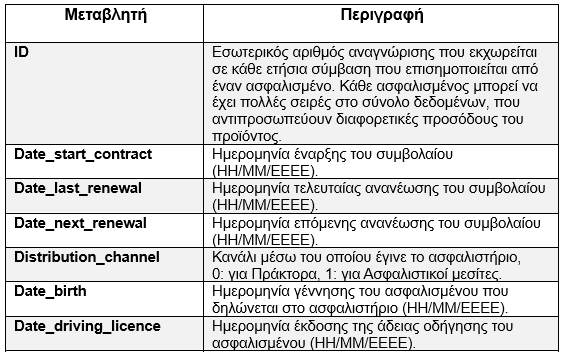
\includegraphics[width=1\textwidth]{images/variables_1.png}
\end{center}

\begin{center}
    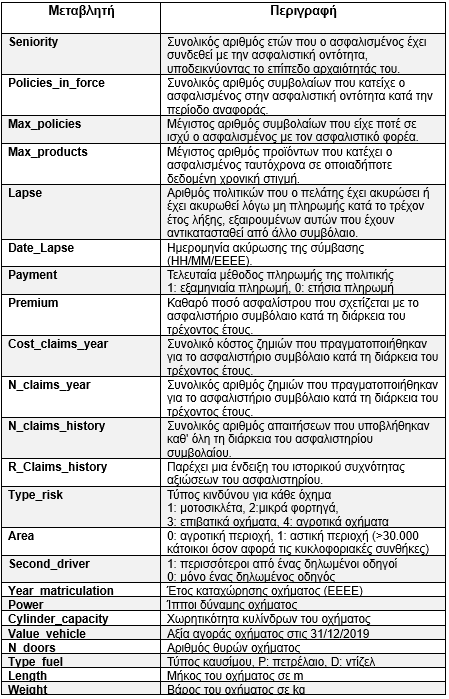
\includegraphics[width=1\textwidth]{images/variables_2.png}
\end{center}

\newpage
\section{Data preproccesing}
Το πρώτο βήμα για την προεπεξεργασία των δεδομένων ήταν να κρατήσουμε μία γραμμή για κάθε 'ID'. Σε ένα 'ID' μπορεί να αντιστοιχούν  περισσότερες από μία γραμμές που αντιπροσωπεύουν το 
ίδιο συμβόλαιο του ίδιου πελάτη για διαφορετική χρονική περίοδο. Έτσι, για κάθε 'ID' κρατάμε την τελευταία ανανέωση του συμβολαίου, δηλαδή την γραμμή με το μεγαλύτερο χρονολογικά 'last\_renewal\_date'. 
Έπειτα, στη θέση του 'premium' υπολογίζουμε και τοποθετούμε τον μέσο όρο των 'premium' όλων των γραμμών με κοινό 'ID'.

Το δεύτερο βήμα ήταν η επεξεργασία όλων των ημερομηνιών. Ειδικότερα, οι στήλες 'Date\_birth', 'Date\_driving\_license', 'Date\_start\_contract', 'Date\_last\_renewal', \\
'Date\_next\_renewal', 'Date\_lapse' δίνονται στην μορφή ΗΗ/ΜΜ/ΕΕΕΕ. Αρχικά, για κάθε μία από αυτές τις μεταβλητές κρατήσαμε το έτος (ΕΕΕΕ) και στην συνέχεια πραγματοποιώντας τις κατάλληλες αφαιρέσεις
δημιουργήσαμε νέες στήλες στο dataset που πήραν την θέση αυτών που αναφέρθηκαν νωρίτερα. Έτσι, δημιουργήσαμε τις στήλες: 'Age' που προσδιορίζει την ηλικία του πελάτη, 'Years\_driving' που προσδιορίζει 
πόσα χρόνια οδηγεί ο πελάτης, 'Year\_on\_road' που προσδιορίζει πόσα χρόνια κυκλοφορεί το κάθε όχημα υπό την κατοχή συγκεκριμένου πελάτη, 'Policy Duration' που υποδεικνύει την διάρκεια του εκάστοτε συμβολαίου σε χρόνια και 
'Years\_on\_policy' που προσδιορίζει πόσα χρόνια ο πελάτης βρίσκεται στον ίδιο τύπο συμβολαίου. Πρέπει να σημειωθεί πως το dataset περιέχει δεδομένα μέχρι και το 2019. Για να έχουμε μια σωστή εικόνα των χρονολογιών
σε όλες αυτές τις μεταβλητές που δημιουργήσαμε, χρησιμοποιήσαμε ως σημείο αναφοράς την χρονολογία τελευταίας ανανέωσης του συμβολαίου. Για παράδειγμα η μεταβλητή 'Age' προκύπτει από την αφαίρεση:
'Age' = 'Date\_last\_renewal' - 'Date\_birth'.

Επιπλέον, δημιουργήσαμε μία ακόμη νέα στήλη με όνομα 'accidents' για να υπάρχει μια συσχέτιση μεταξύ των αριθμών των ατυχημάτων με τα χρόνια που ένας πελάτης είναι ασφαλισμένος στην εταιρεία.

Διαχειριστήκαμε την απουσία τιμών με δύο τρόπους. Στην στήλη 'Length' αντικαταστήσαμε τα κενά πεδία με τον μέσο όρο των τιμών της στήλης. Στην στήλη 'Type\_fuel' αντικαταστήσαμε τα κενά πεδία με την τιμή 
'Unknown'.

Μετά από δοκιμές διαπιστώσαμε πως κάποιες μεταβλητές του dataset δεν συνεισέφεραν καθόλου στην βελτίωση της απόδοσης και παραλείφθηκαν. Οι στήλες που χρησιμοποιήθηκαν τελικά είναι οι: 
'Seniority', 'Premium', 'Type\_risk', 'Area', 'Power', 'Second\_driver', 'Years\_on\_road', 'R\_claims\_history', 'Years\_on\_policy', 'accidents', 'Value\_vehicle, 'Age', 'Years\_driving', 'Distribution\_channel', 'N\_claims\_history',
\\ 'Cylinder\_capacity', 'Weight', 'Length', 'Type\_fuel', 'Payment', 'Contract\_year', \\'Policies\_in\_force', 'Lapse'.

\section{Διαγράμματα}
Τα διαγραμματα
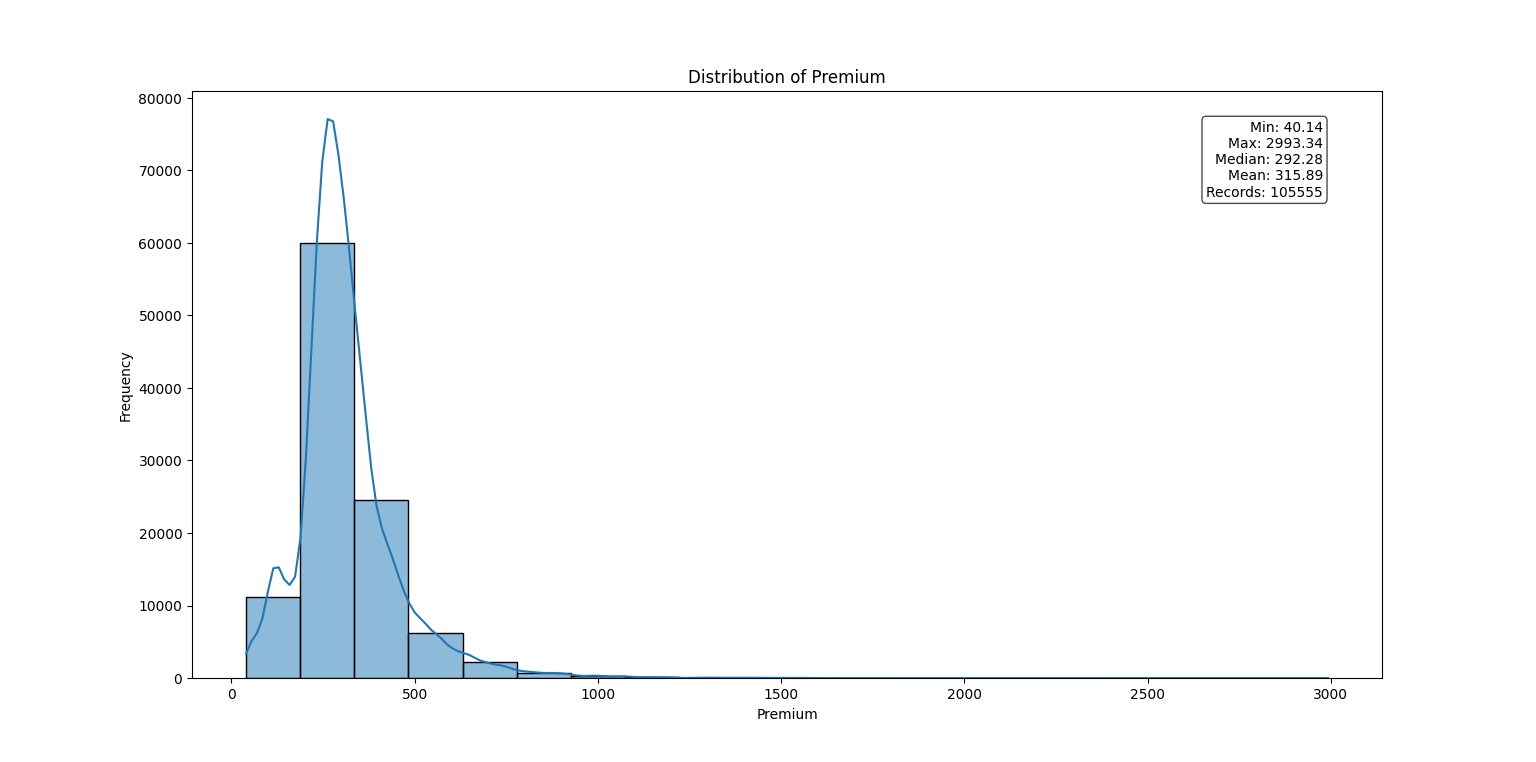
\includegraphics[width=1\textwidth, keepaspectratio]{images/premium.png}

\begin{figure}
    \centering
     \begin{subfigure}{0.45\linewidth}
      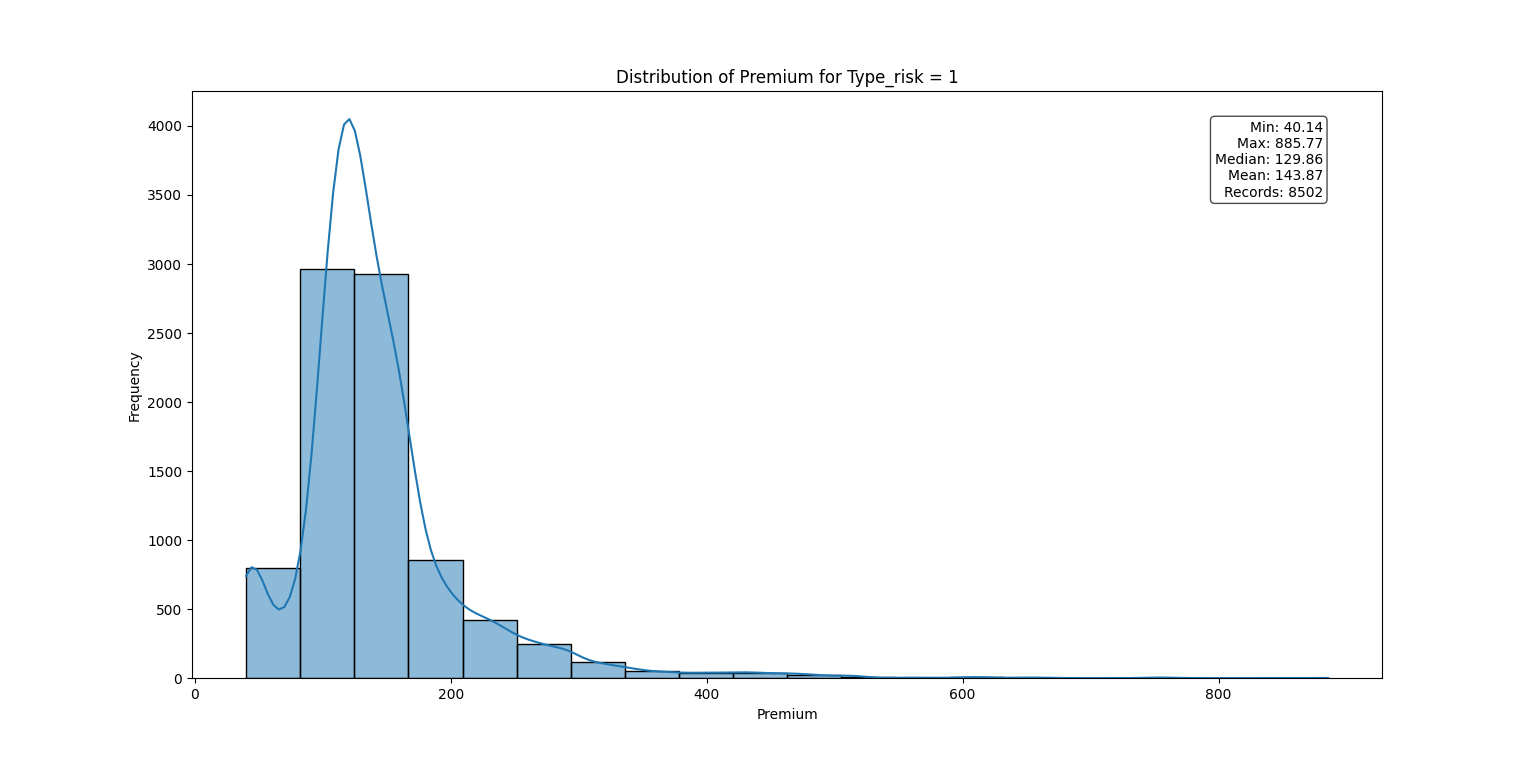
\includegraphics[width=\linewidth]{images/premium_risk1.png}
      \caption{Motorbikes}
      \label{fig:subfig1}
     \end{subfigure}
     \begin{subfigure}{0.45\linewidth}
      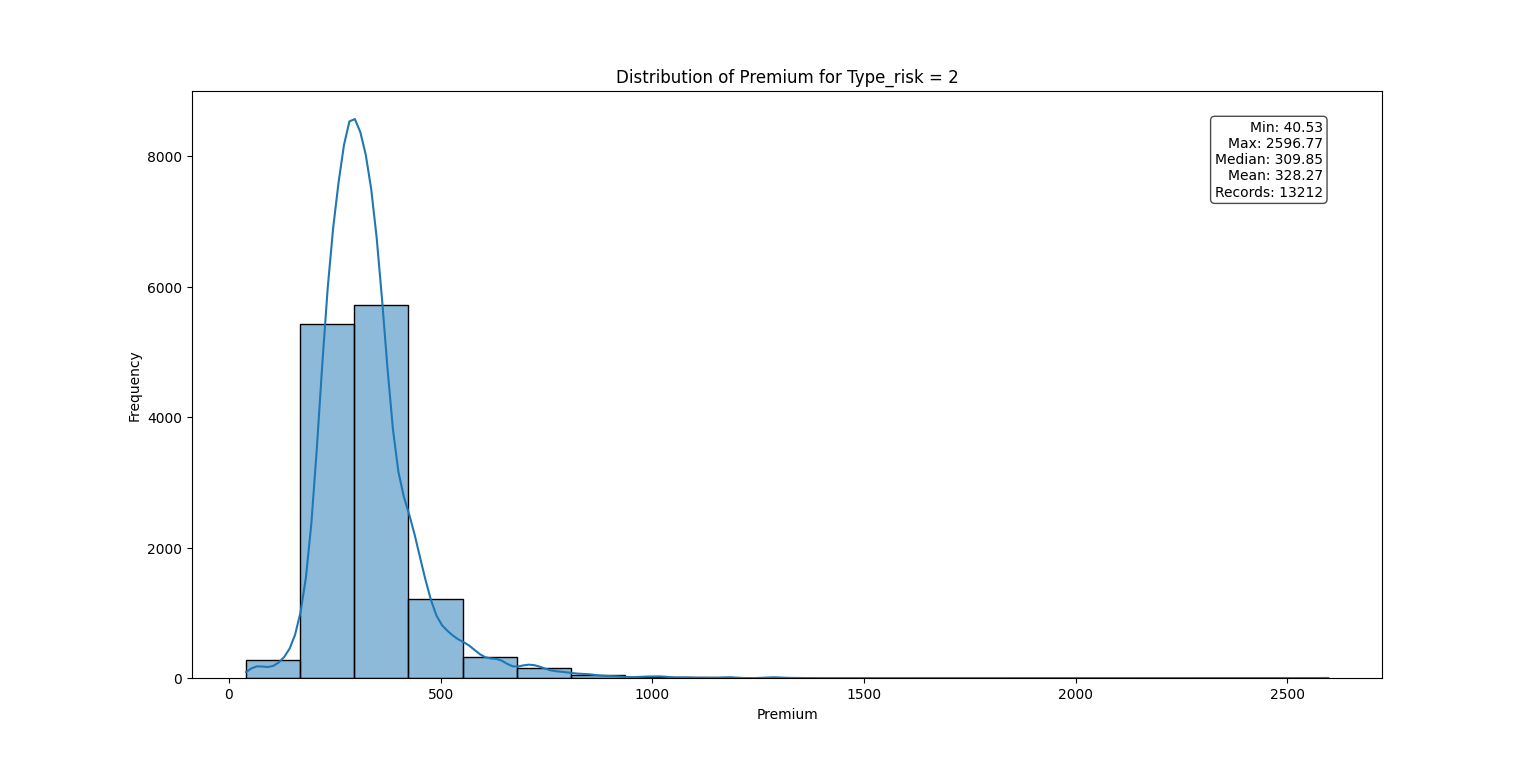
\includegraphics[width=\linewidth]{images/premium_risk2.png}
      \caption{Vans}
      \label{fig:subfig2}
      \end{subfigure}
  \vfill
       \begin{subfigure}{0.45\linewidth}
       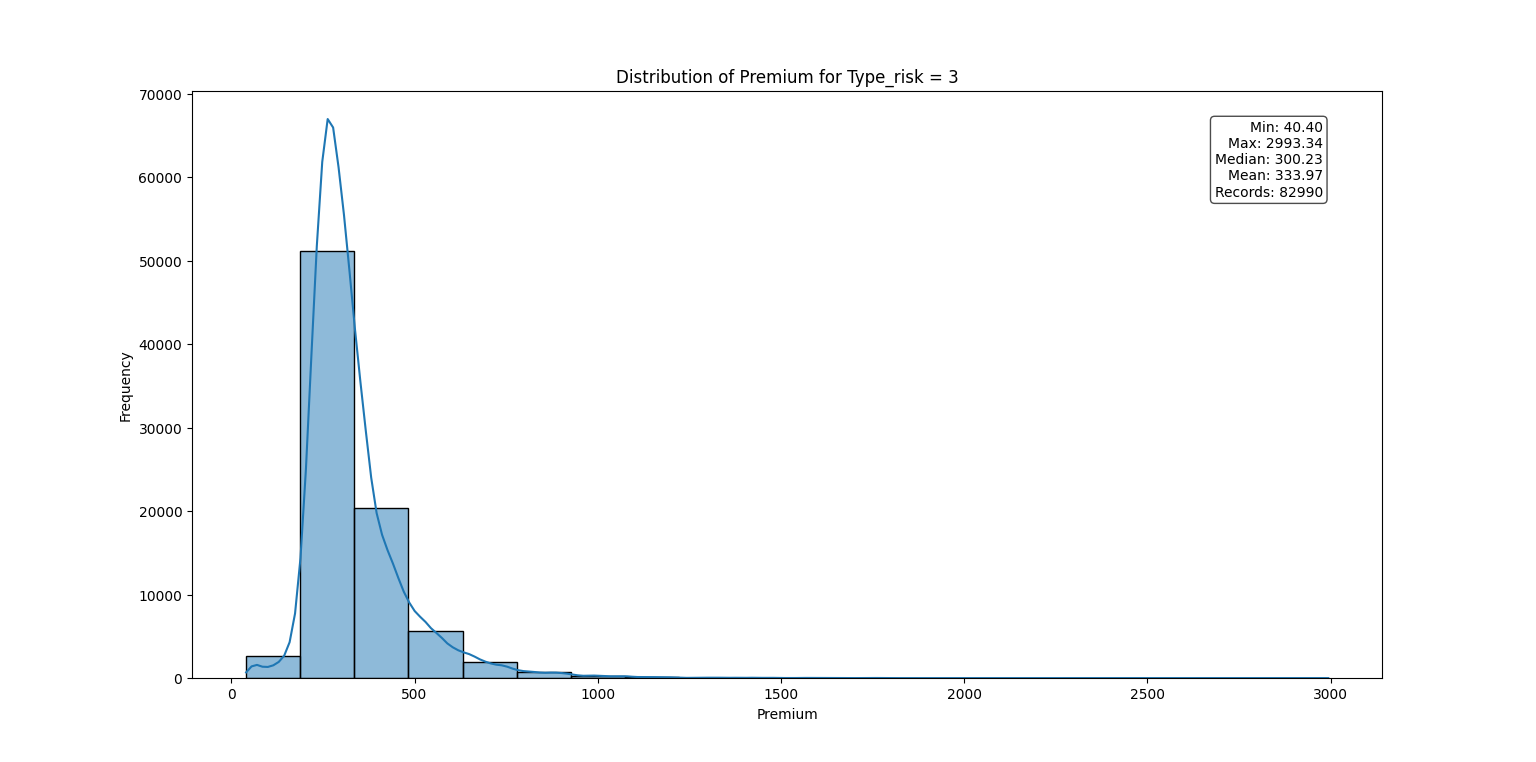
\includegraphics[width=\linewidth]{images/premium_risk3.png}
       \caption{Passenger cars}
       \label{fig:subfig3}
        \end{subfigure}
         \begin{subfigure}{0.45\linewidth}
        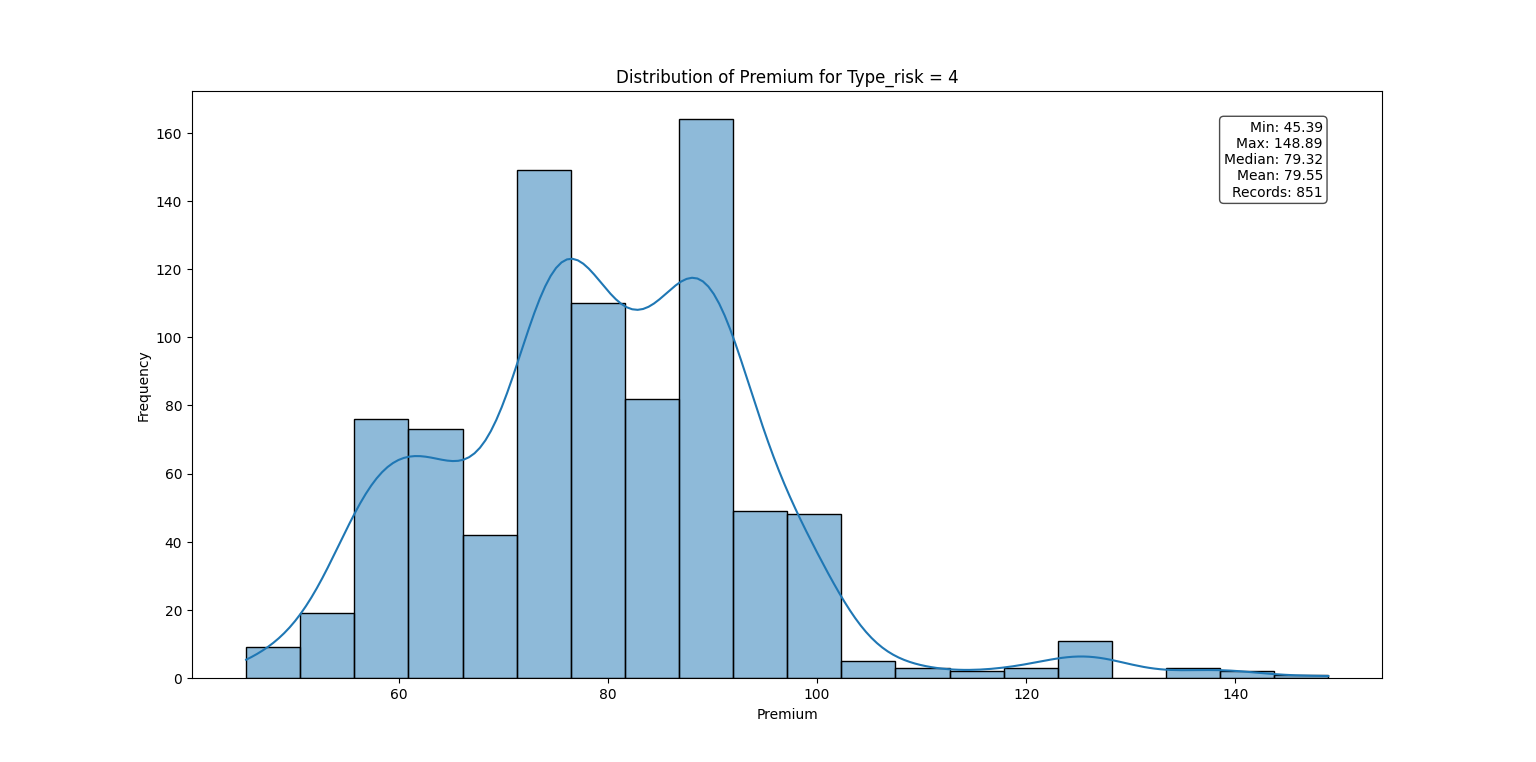
\includegraphics[width=\linewidth]{images/premium_risk4.png}
        \caption{Agricultural Vehicles}
        \label{fig:subfig4}
         \end{subfigure}
  \caption{Comparison of Different Vehicle Types}
  \label{fig:subfigures4}
\end{figure}


\begin{observation}
    Στο πρώτο διάγραμμα παρουσιάζεται η κατανομή των ασφαλίστρων για όλες τις καταχωρίσεις. Τα επόμενα διαγράμματα δείχνουν την κατανομή των ασφαλίστρων για κάθε κατηγορία οχημάτων ξεχωριστά.

    Εύκολα διαπιστώνεται από το πρώτο ολικό διάγραμμα ότι οι ασφαλιστικές τιμές πάνω από 500 είναι ελάχιστες και δεν επηρεάζουν σημαντικά το τελικό αποτέλεσμα. Ωστόσο, όταν κατηγοριοποιήσαμε τα δεδομένα, παρατηρήσαμε ότι η διασπορά των τιμών στα αγροτικά οχήματα ήταν μεγαλύτερη, με αποτέλεσμα η διαφοροποίηση του μοντέλου ανά κατηγορία οχήματος να είναι απαραίτητη.
\end{observation}

\section{User Interface}
Το user interface της εφαρμογής αναπτύχθηκε με χρήση της Python και ειδικότερα του framework Kivy, καθώς και της συλλογής από γραφικά στοιχεία KivyMD. Στην εφαρμογή μας υπάρχουν πέντε διαφορετικές "οθόνες".
\begin{enumerate}
    \item Η οθόνη του login
    \item Η οθόνη συμπλήρωσης στοιχείων του πελάτη που πρόκειται να ασφαλίσει το όχημά του.
    \item Η οθόνη συμπλήρωσης στοιχείων του οχήματος που πρόκειται να ασφαλιστεί.
    \item Η οθόνη συμπλήρωσης στοιχείων παλαιότερων συμβολαίων που είχε ο πελάτης στην εταιρεία.
    \item Η οθόνη παρουσίασης της προτεινόμενης ετήσιας τιμής χρέωσης του πελάτη με βάση τα στοιχεία που συμπληρώθηκαν.
\end{enumerate}

\subsection{Login}
\begin{figure}
    \begin{center}
        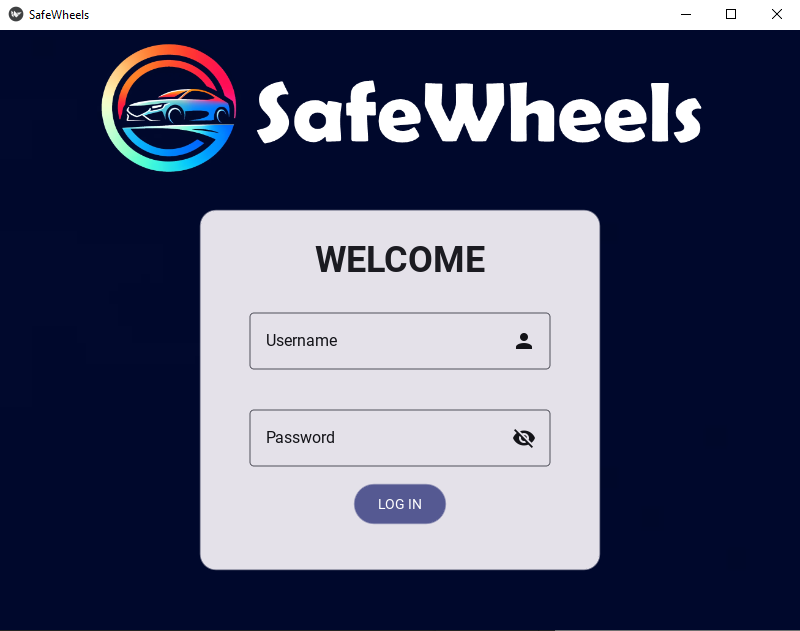
\includegraphics[width=0.7\textwidth]{images/login.png}
    \end{center}
    \caption{Οθόνη login}    
\end{figure}


Πρόκειται για την αρχική οθόνη της εφαρμογής στην οποία ο χρήστης-υπάλληλος της εταιρείας θα πρέπει να συμπληρώσει τα σωστά στοιχεία συνδεσής του (username και password) και στην συνέχεια να πατήσει το κουμπί "LOG IN". Σε περίπτωση που ένα από τα δύο πεδία μείνει κενό, ο χρήστης θα λάβει το αντίστοιχο μήνυμα λάθους [Εικ. \ref{fig:empty}].
Σε περίπτωση που τα στοιχεία σύνδεσης δεν είναι σωστά, ο χρήστης θα λάβει διαφορετικό μήνυμα λάθους [Εικ. \ref{fig:match}].

Έχει προβλεφθεί και δημιοθργηθεί μόνο ένας λογαριασμός υπαλλήλου. 'Ετσι, για να πάμε στην επόμενη οθόνη θα πρέπει να συμπληρώσουμε στο πεδίο username: \textbf{admin\_1} και στο πεδίο password: \textbf{12345}. Αφού συμπληρώσουμε αυτά τα στοιχεία σωστά και πατήσουμε το κουμπί "LOG IN" μεταφερόμαστε στην δεύτερη οθόνη.

\begin{figure}
    \centering
    \begin{subfigure}{0.45\linewidth}
        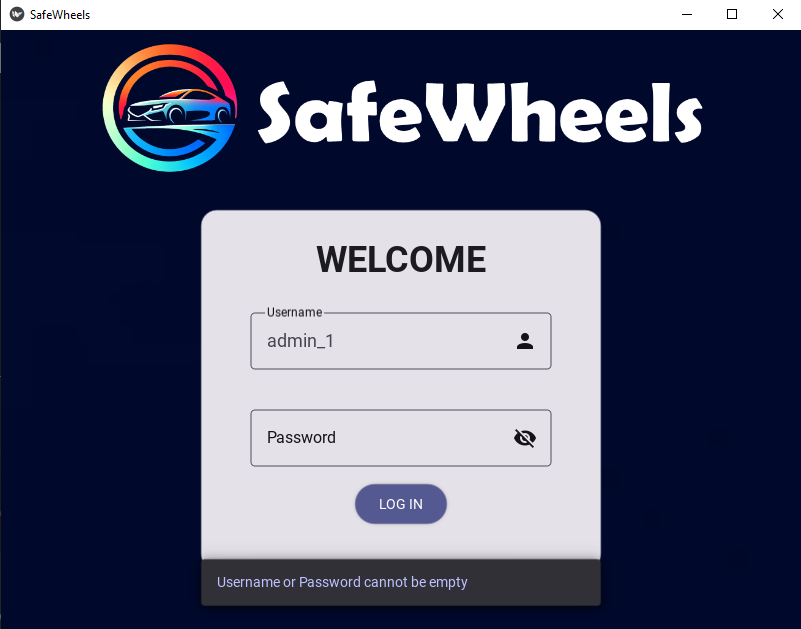
\includegraphics[width=\linewidth]{images/login_empty.png}
        \caption{Κενό πεδίο}
        \label{fig:empty}
    \end{subfigure}
    \begin{subfigure}{0.45\linewidth}
        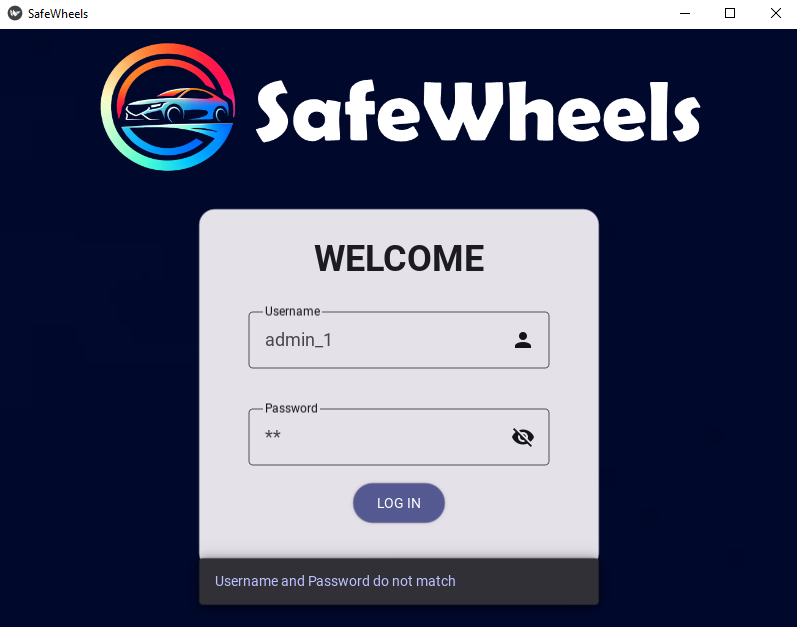
\includegraphics[width=\linewidth]{images/login_dont_match.png}
        \caption{Λάθος στοιχεία}
        \label{fig:match}
    \end{subfigure}
    \caption{Μηνύματα λάθους στο login}
    \label{fig:errors}
\end{figure}
        
   

\end{document}

